\section[Considérations pratiques et résultats]{Considérations pratiques et résultats}
\subsection{En pratique}

\begin{frame}{Implémentation}
\begin{itemize}
  \item Cœur du projet en \textbf{C} : traitement, calculs, reconstruction.
\end{itemize}
\pause
\vspace{0.5em}
\tiny{
\renewcommand{\arraystretch}{1.5} % augmente l’espacement vertical
\setlength{\tabcolsep}{4pt} % réduit l’espacement horizontal des colonnes
\begin{tabular}{|>{\ttfamily}l|p{8cm}|}
\hline
\textbf{Fichier} & \textbf{Rôle} \\
\hline
matrice.c & Implémente les opérations sur les matrices. \\
\hline
selection.c & Sélectionne des points d'intérêt. \\
\hline
trouve\_coin.c & Raffine les points détectés. \\
\hline
ransac.c & Second raffinement des points par RANSAC. \\
\hline
appariement.c & Calcule le descripteur BRIEF et la distance à la droite épipolaire. \\
\hline
detection.c & Regroupe détection, tri et appariement pour un couple d’images. \\
\hline
camera\_calibration.c & Calibre la caméra à partir des correspondances 2D. \\
\hline
SVD.c & Fonctions pour la décomposition SVD et résolution de systèmes. \\
\hline
reconstruction.c & Reconstruit les coordonnées 3D à partir des points 2D. \\
\hline
triangles.c & Détermine les triangles pour reconstruire l'enveloppe 3D. \\
\hline
manipulation\_fichier.c & Utilitaires de lecture/écriture de matrices. \\
\hline
constante.c & Gère les paramètres de reconstruction. \\
\hline
\end{tabular}
}
\pause
\normalsize
\vspace{0.5em}
\begin{itemize}
  \item Interface utilisateur et affichage en \textbf{Python}.
\end{itemize}
\end{frame}


\begin{frame}{Shooting photo : importance de la prise de vue}
  \note{
    au depart : on tourne autour/ faire tourner rubiks 
    fond unis mieux pour la Calibration
    face recouverte de papier pour etre unis et limiter les points inutiles
  }
  \centering
  \begin{minipage}{0.48\linewidth}
    \centering
    \begin{figure}
      \centering
      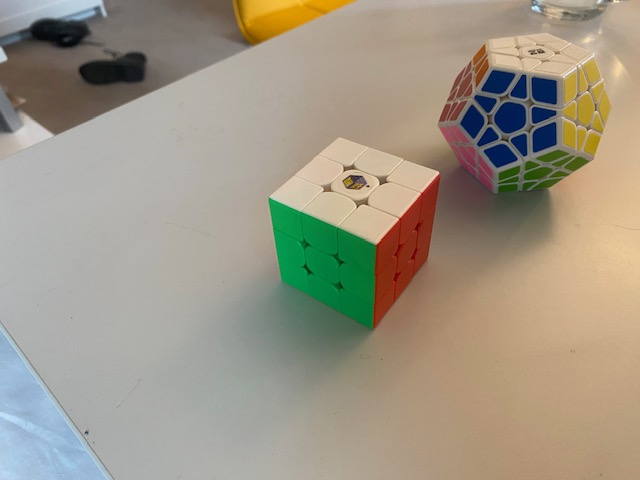
\includegraphics[width=0.48\linewidth]{capture/dodec0.jpg}%
      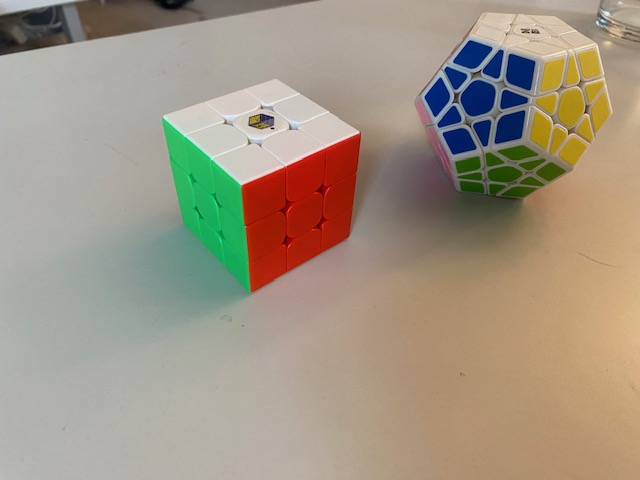
\includegraphics[width=0.48\linewidth]{capture/dodec1.jpg} \\
      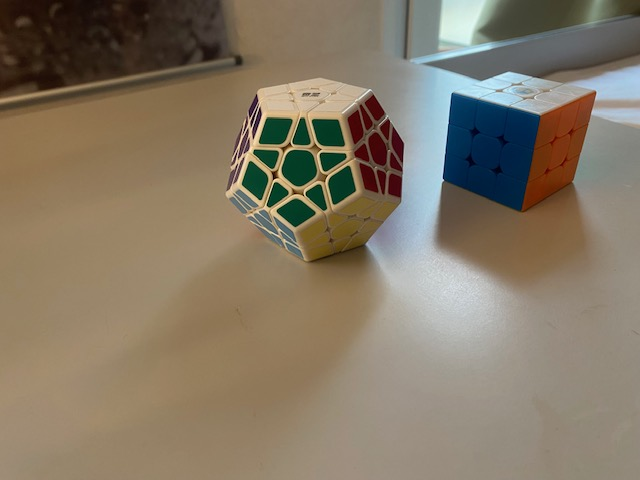
\includegraphics[width=0.48\linewidth]{capture/dodec2.jpg}%
      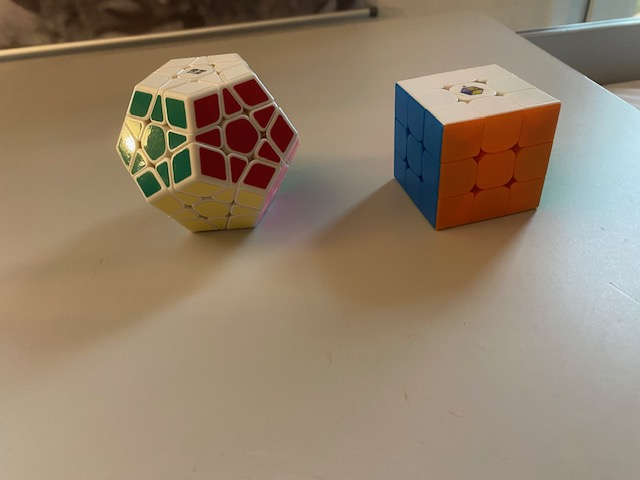
\includegraphics[width=0.48\linewidth]{capture/dodec3.jpg}
      {\footnotesize\textbf{Vues initiales}}
    \end{figure}
  \end{minipage}
  \hfill
  \begin{minipage}{0.48\linewidth}
    \centering
    \begin{figure}
      \centering
      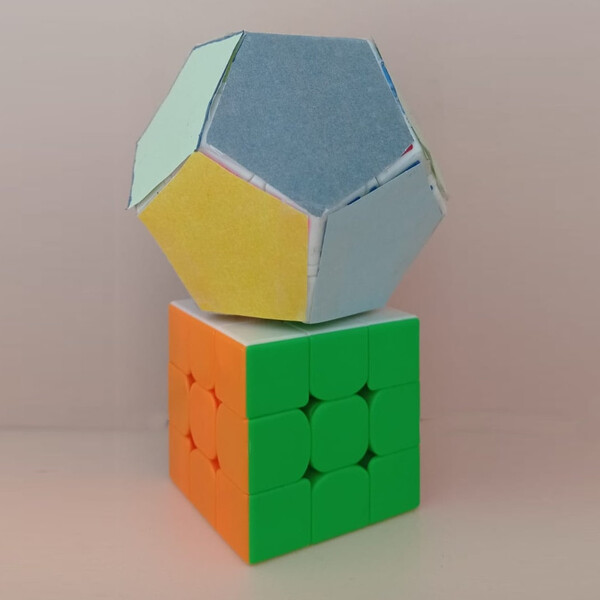
\includegraphics[width=0.48\linewidth]{capture/dodecf0.jpg}%
      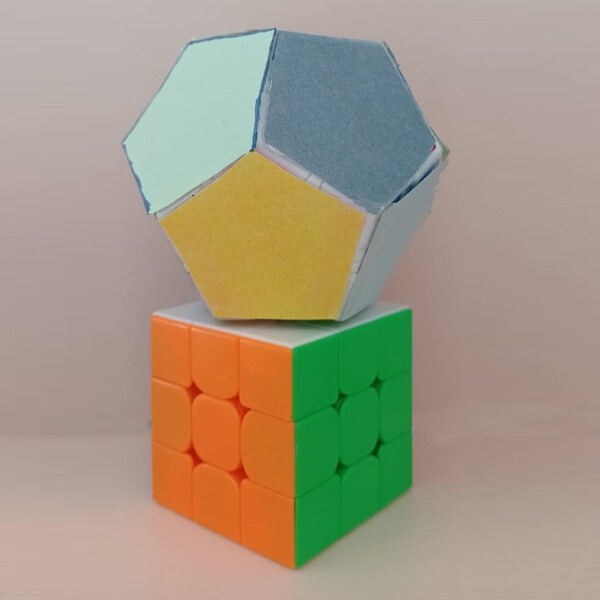
\includegraphics[width=0.48\linewidth]{capture/dodecf1.jpg} \\
      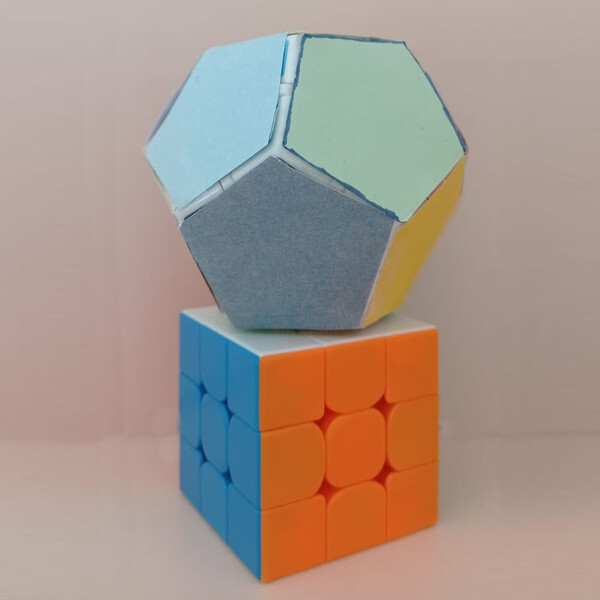
\includegraphics[width=0.48\linewidth]{capture/dodecf2.jpg}%
      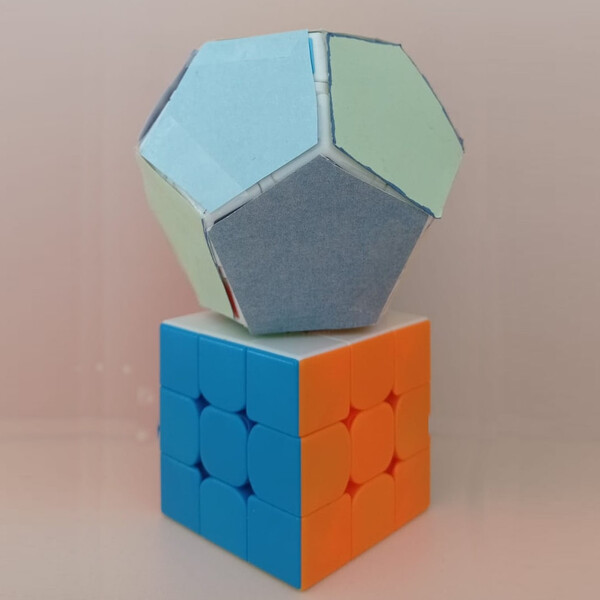
\includegraphics[width=0.48\linewidth]{capture/dodecf3.jpg}
      {\footnotesize\textbf{Vues améliorées}}
    \end{figure}
  \end{minipage}
\end{frame}


%------------------------------------------------
\subsection{Quelques exemples}
%------------------------------------------------

\begin{frame}{Le dodécahèdre}
\begin{minipage}{0.40\textwidth}
    \centering
    \setlength{\tabcolsep}{0pt}
    \renewcommand{\arraystretch}{0}
    \begin{tabular}{cc}
        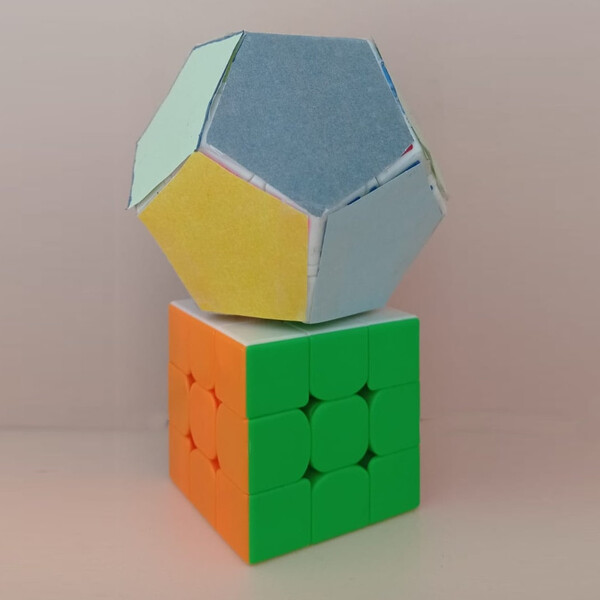
\includegraphics[width=0.36\textwidth]{capture/dodecf0.jpg} &
        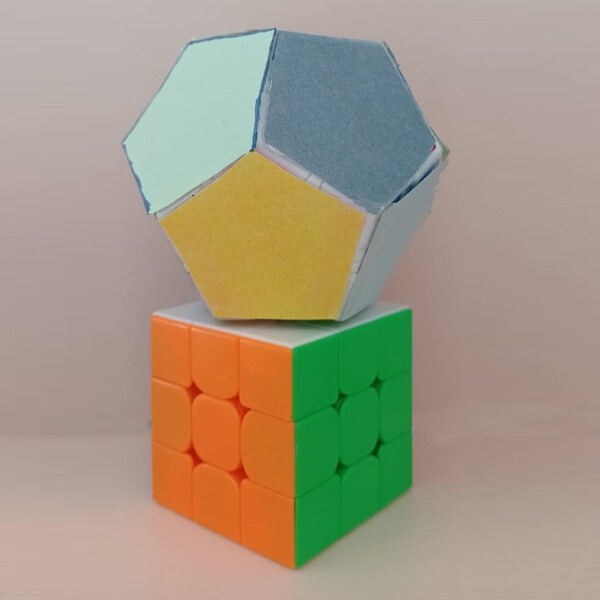
\includegraphics[width=0.36\textwidth]{capture/dodecf1.jpg} \\
        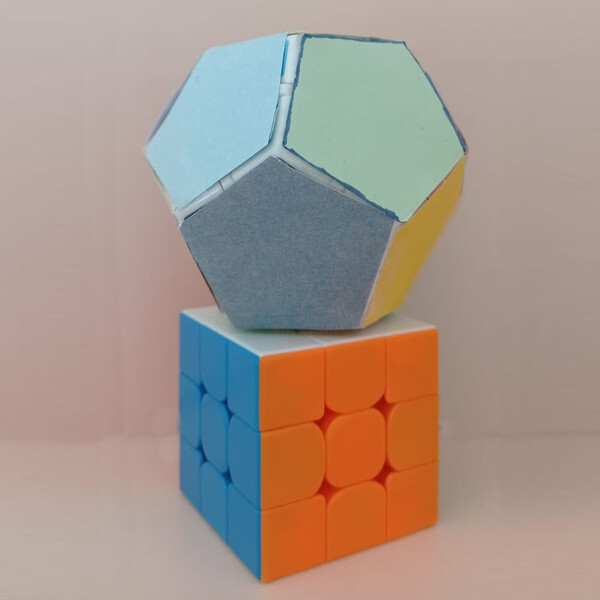
\includegraphics[width=0.36\textwidth]{capture/dodecf2.jpg} &
        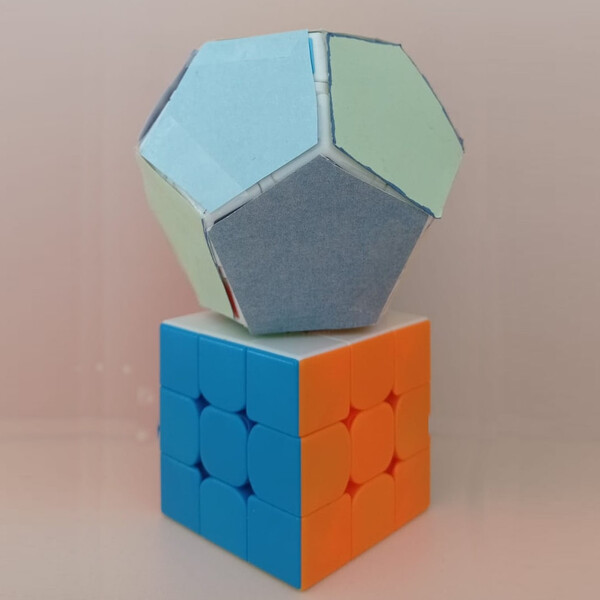
\includegraphics[width=0.36\textwidth]{capture/dodecf3.jpg} \\
        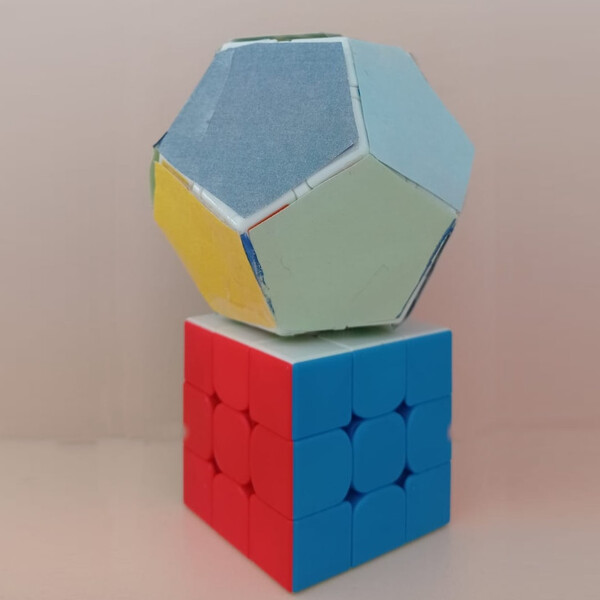
\includegraphics[width=0.36\textwidth]{capture/dodecf4.jpg} &
        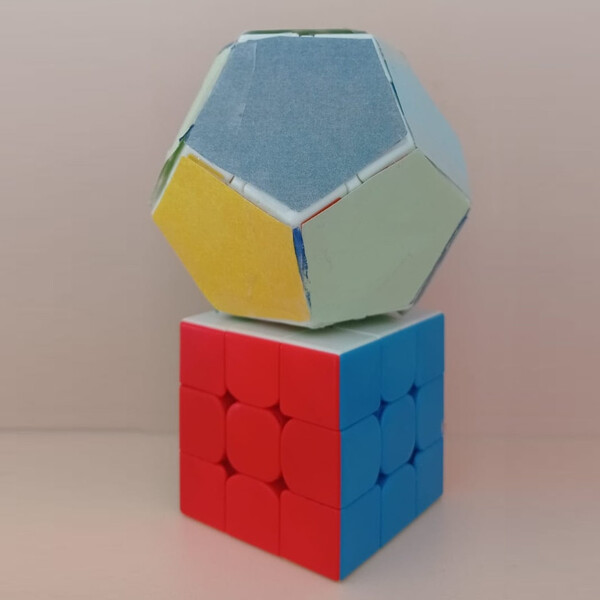
\includegraphics[width=0.36\textwidth]{capture/dodecf5.jpg} \\
        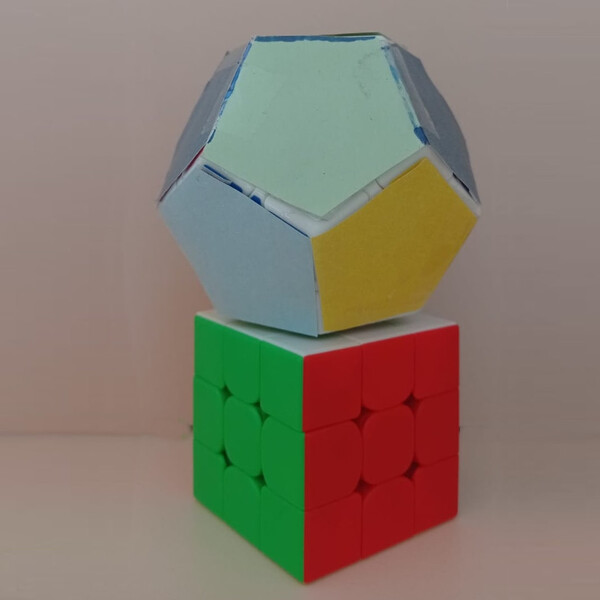
\includegraphics[width=0.36\textwidth]{capture/dodecf6.jpg} &
        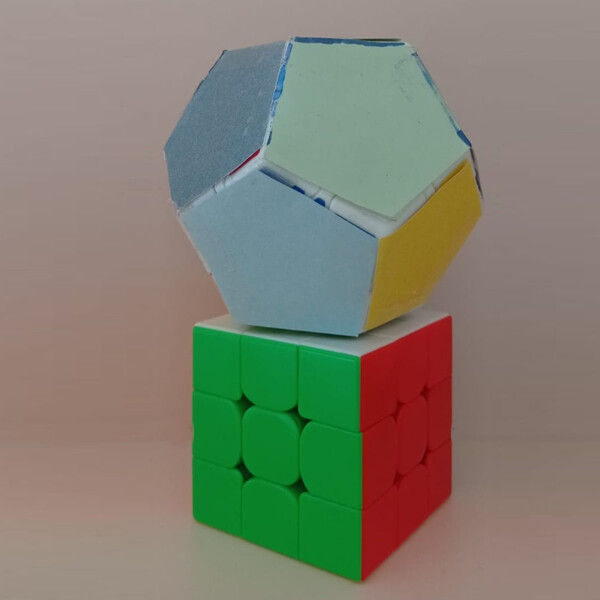
\includegraphics[width=0.36\textwidth]{capture/dodecf7.jpg} \\
    \end{tabular}
\end{minipage}%
\hfill
\begin{minipage}{0.60\textwidth}
    \centering
    \setlength{\tabcolsep}{0pt}
    \renewcommand{\arraystretch}{0}
    \begin{tabular}{c}
        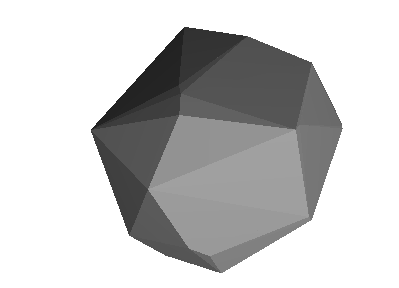
\includegraphics[width=0.72\textwidth]{capture/dodec_vrai.png} \\
    \end{tabular}
    \vspace{0.5em}

    {\tiny \textit{visualisation sur viewstl.com}}
\end{minipage}
\end{frame}


\begin{frame}{La pyramide}
\begin{minipage}{0.40\textwidth}
    \centering
    \setlength{\tabcolsep}{0pt}
    \renewcommand{\arraystretch}{0}
    \begin{tabular}{cc}
        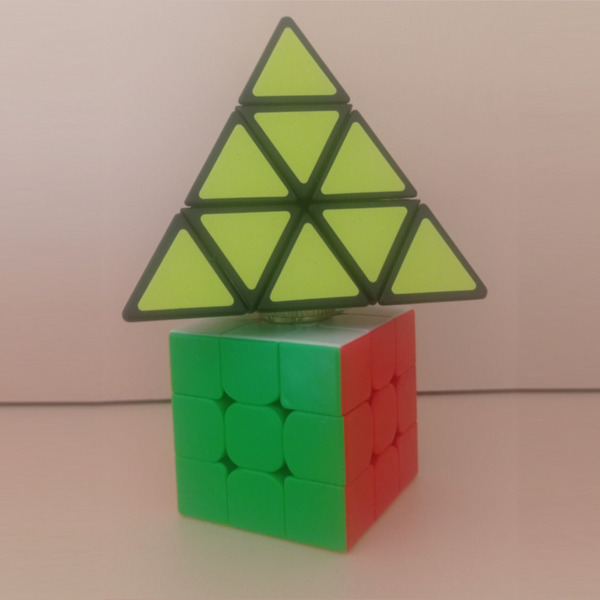
\includegraphics[width=0.36\textwidth]{capture/pyra0.jpg} &
        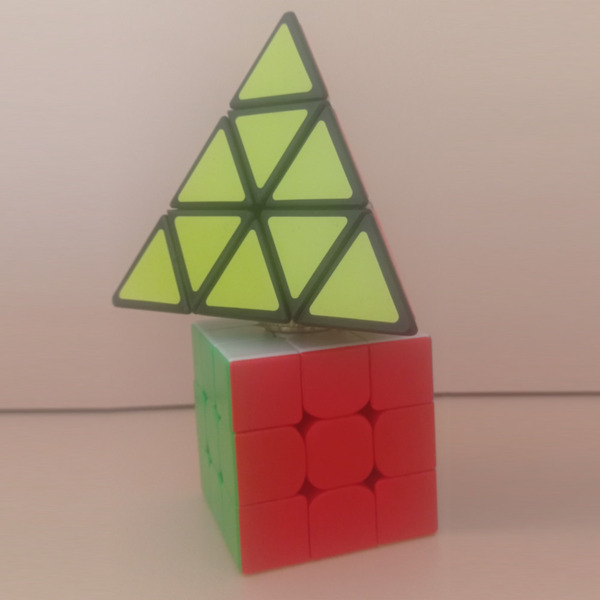
\includegraphics[width=0.36\textwidth]{capture/pyra1.jpg} \\ 
        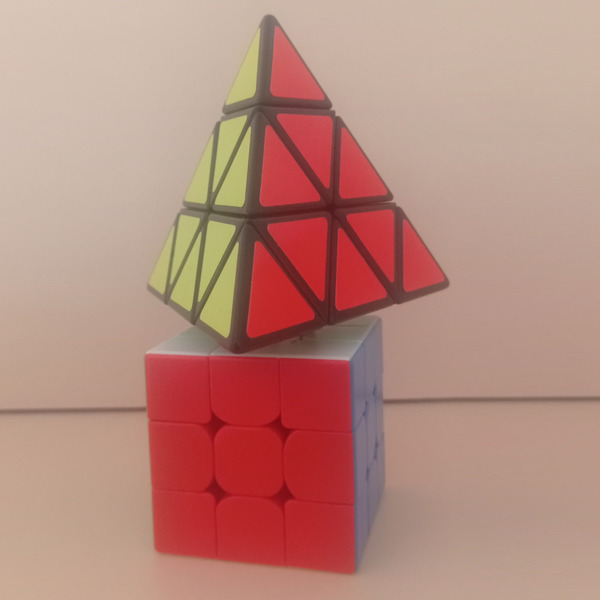
\includegraphics[width=0.36\textwidth]{capture/pyra2.jpg} &
        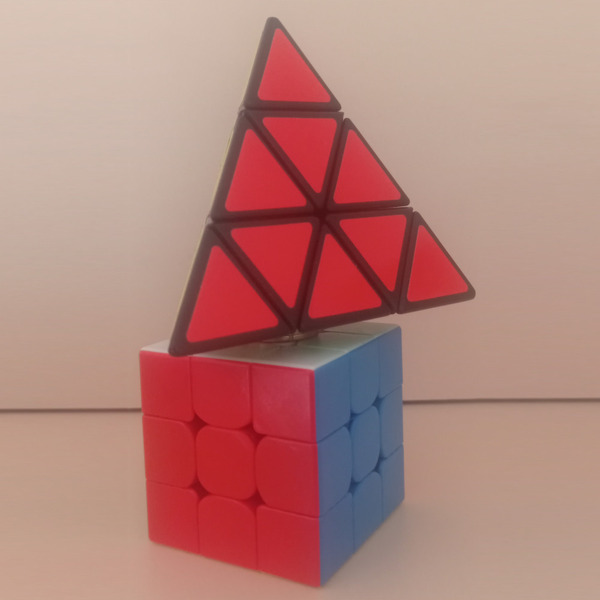
\includegraphics[width=0.36\textwidth]{capture/pyra3.jpg} \\
        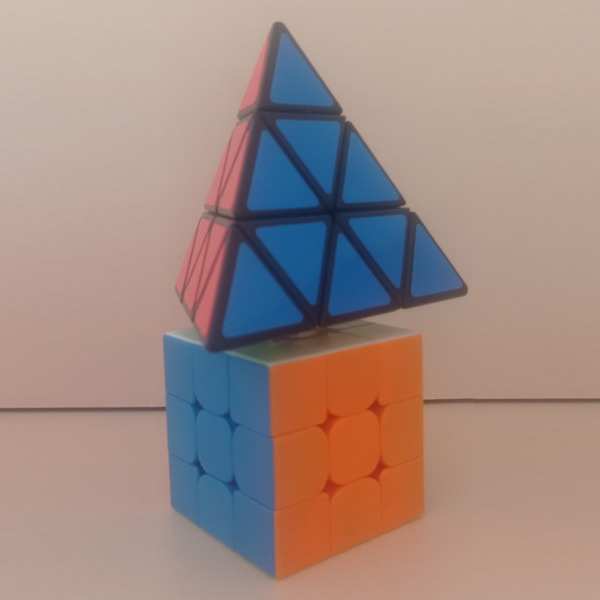
\includegraphics[width=0.36\textwidth]{capture/pyra4.jpg} &
        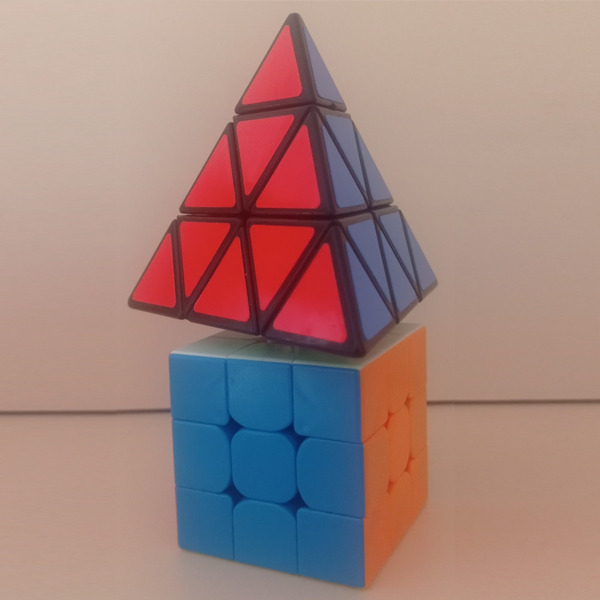
\includegraphics[width=0.36\textwidth]{capture/pyra5.jpg} \\
        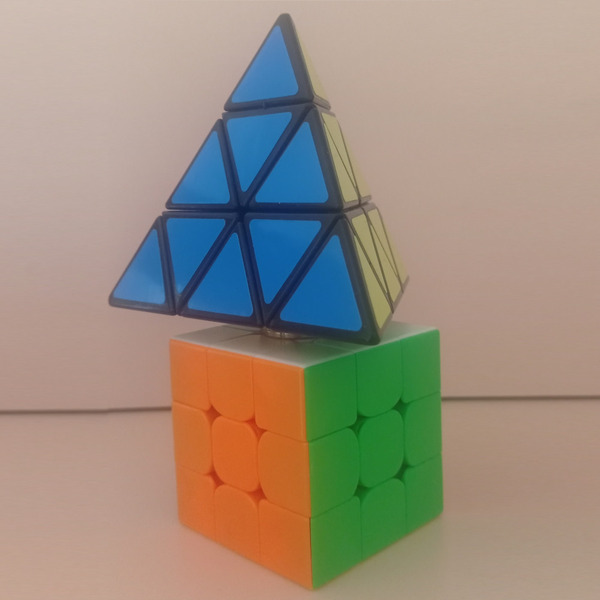
\includegraphics[width=0.36\textwidth]{capture/pyra6.jpg} &
        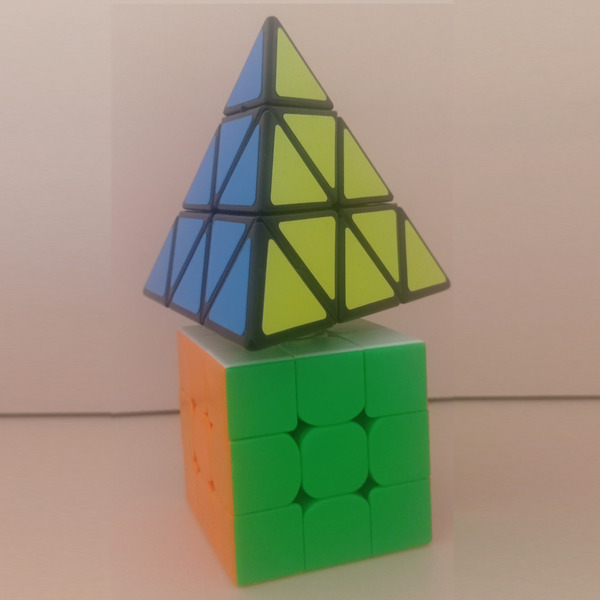
\includegraphics[width=0.36\textwidth]{capture/pyra7.jpg} \\
    \end{tabular}
\end{minipage}%
\hfill
\begin{minipage}{0.60\textwidth}
    \centering
    \setlength{\tabcolsep}{0pt}
    \renewcommand{\arraystretch}{0}
    \begin{tabular}{cc}
        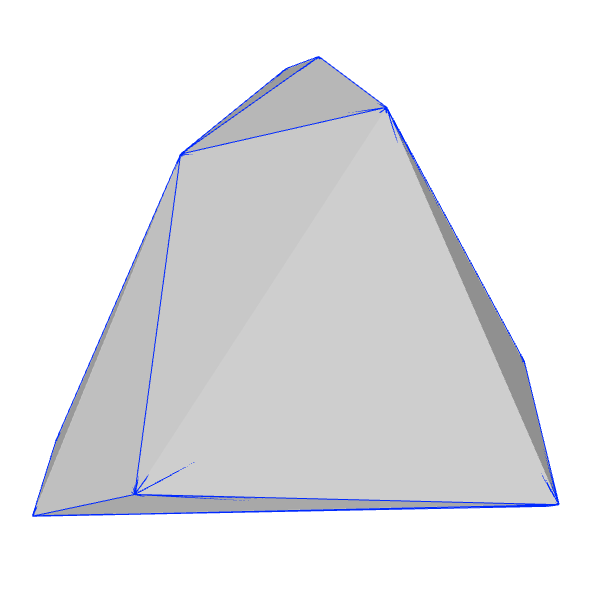
\includegraphics[width=0.40\textwidth]{capture/face1.png} &
        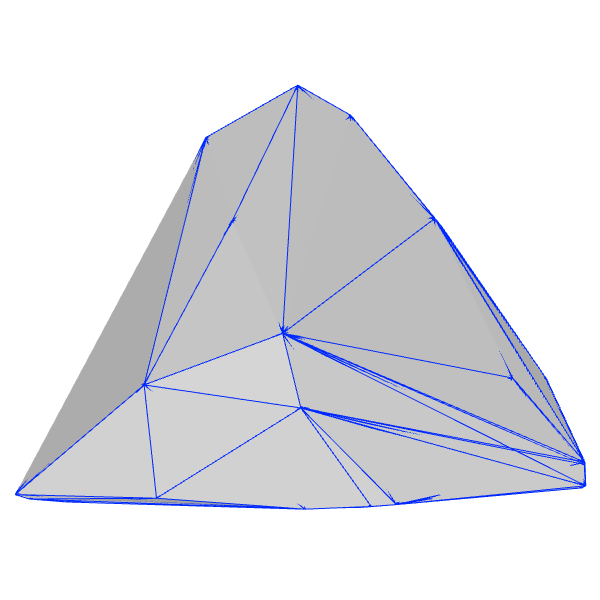
\includegraphics[width=0.40\textwidth]{capture/face2.png} \\
        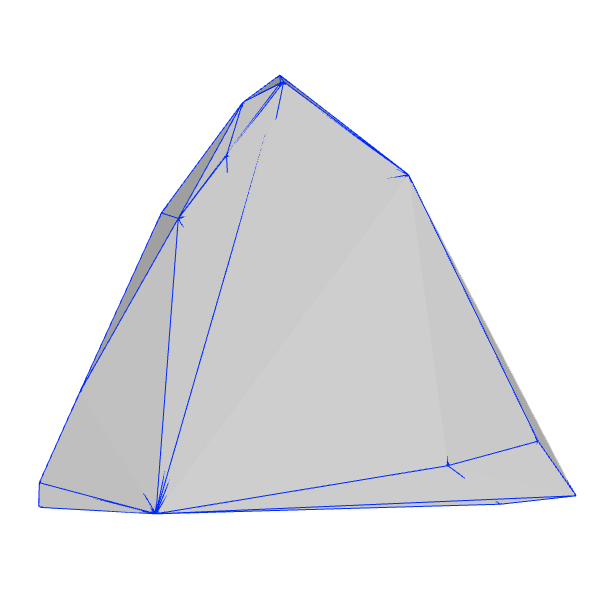
\includegraphics[width=0.40\textwidth]{capture/face3.png} &
        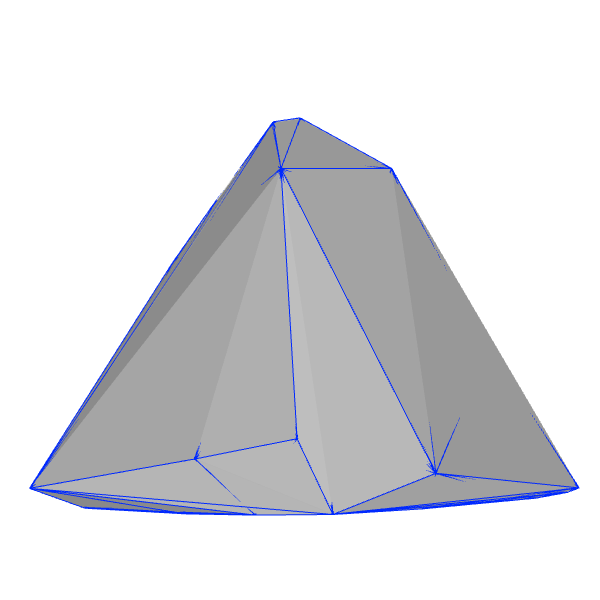
\includegraphics[width=0.40\textwidth]{capture/profil.png} \\
    \end{tabular}
    \vspace{0.2em}

    {\tiny \textit{visualisation sur 3dviewer.net}}
\end{minipage}
\end{frame}

%++++++++++++++++++++++++++++++++++++++++++++++++
\subsection{Des pistes d'amélioration}

%------------------------------------------------

%++++++++++++++++++++++++++++++++++++++++++++++++
\subsection{Limite de la méthode}

%------------------------------------------------
\begin{frame}{Une importante sensibilité aux erreurs}
\centering
\begin{minipage}{0.45\textwidth}
    \centering
    \begin{tikzpicture}
      \node[anchor=south west, inner sep=0] (img1) at (0,0) {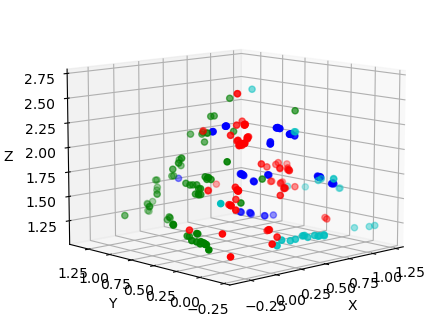
\includegraphics[width=\linewidth]{capture/reconstruit_pyra.png}};
        \begin{scope}[x={(img1.south east)}, y={(img1.north west)}]
            \draw[red, thick] (0.28,0.35) circle [radius=0.03]; % Ajuste les coordonnées
        \end{scope}
    \end{tikzpicture}
    
    \vspace{0.3em}

    \small\textit{points localisés par le programme}
\end{minipage}
\hfill
\begin{minipage}{0.45\textwidth}
    \centering
    \begin{tikzpicture}
      \node[anchor=south west, inner sep=0] (img1) at (0,0) {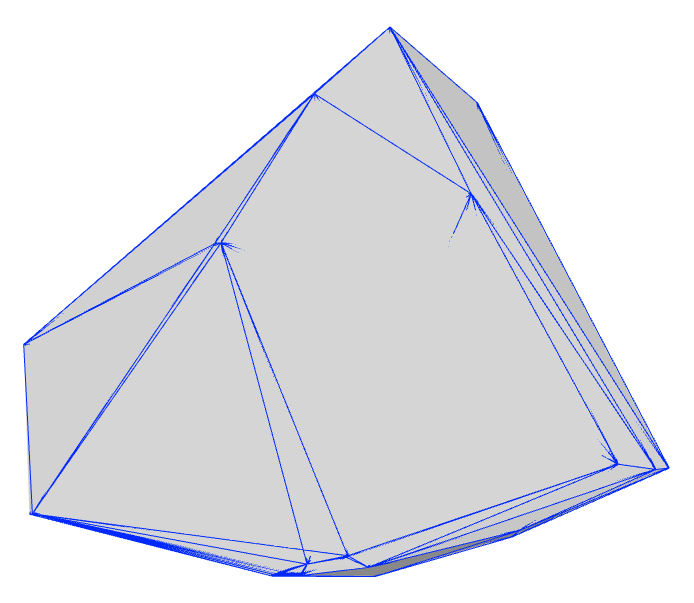
\includegraphics[width=\linewidth]{capture/erreur.png}};
        \begin{scope}[x={(img1.south east)}, y={(img1.north west)}]
            \draw[red, thick] (0.04,0.42) circle [radius=0.03]; % Ajuste les coordonnées
        \end{scope}
    \end{tikzpicture}
    
    \vspace{0.3em}
  \begin{flushleft}
    \small\textit{enveloppe convexe visualisé avec 3dview.net}
  \end{flushleft}

\end{minipage}
\end{frame}